%\setlength{\belowdisplayskip}{3pt} \setlength{\belowdisplayshortskip}{3pt}
%\setlength{\abovedisplayskip}{3pt} \setlength{\abovedisplayshortskip}{3pt}

\begin{figure*}[!t]
\centering
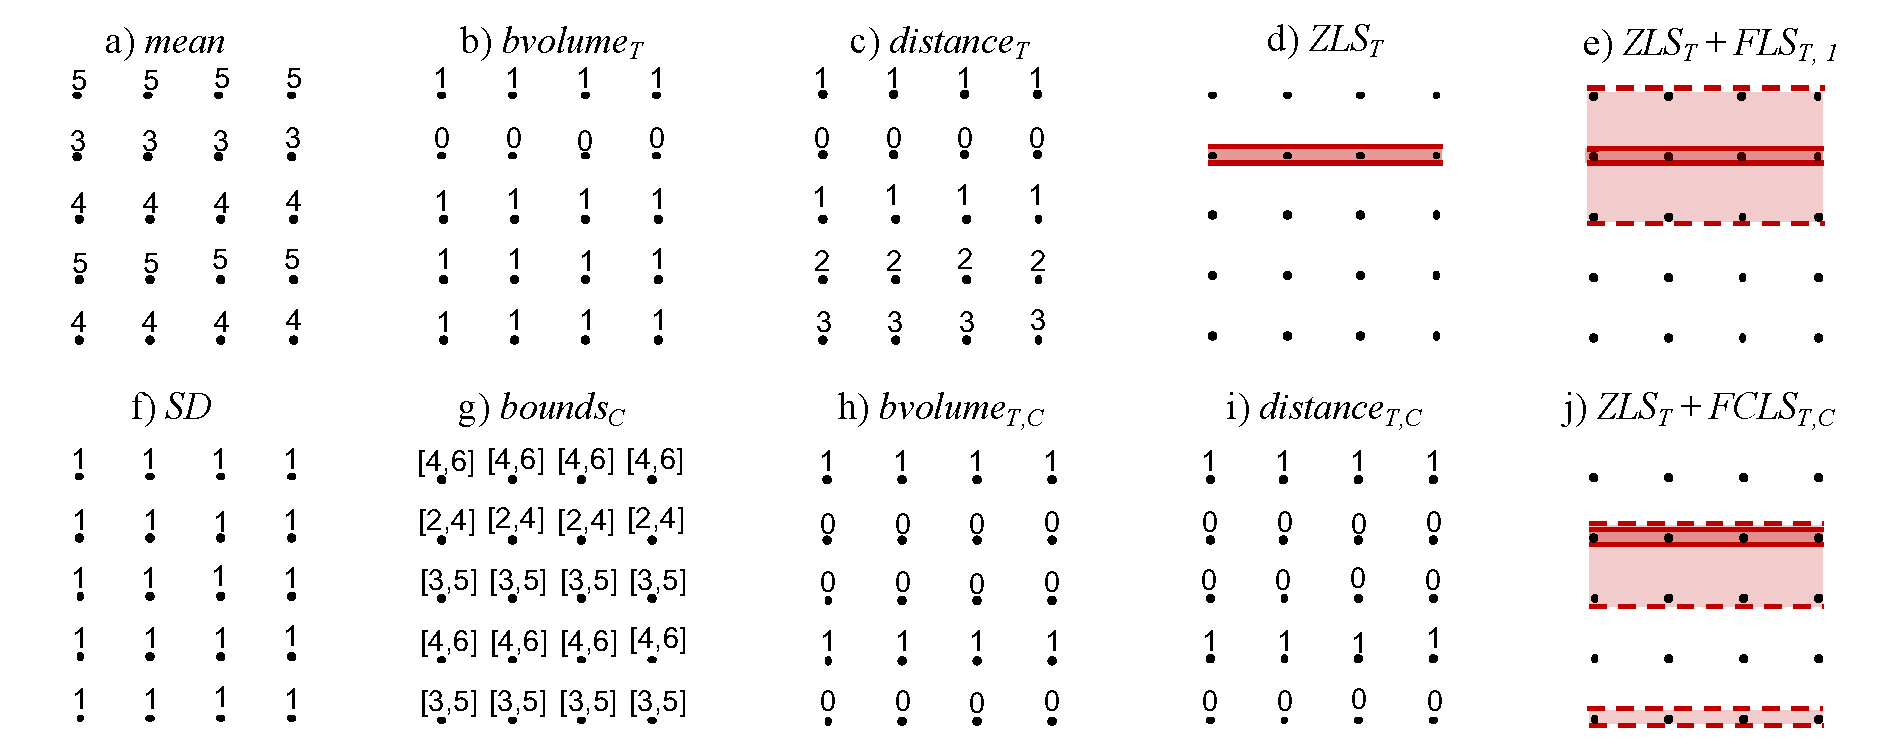
\includegraphics[width=\linewidth]{Images/example.pdf}
\vspace{-5mm}
\caption{A notional example showing the steps involved in generating feature level-sets $FLS_{T}$ and feature confidence level-set $FCLS_{T,C}$ for an uncertain univariate field represented using $mean$~(a) and $SD$~(f). For this example, we use trait $T=[2.5, 3.5]$ and confidence $C=68\%$, i.e., $Z=1$. The top row~(b-e) shows the steps to compute $FLS_{T}$. The bottom row~(g-j) shows the steps to compute $FCLS_{T}$. $ZLS_{T}$ represents the ``zero'' level-set extracted using $distance_{T}$.}
% In comparison to using $FLS_{T}$, for uncertain multivariate data, by leveraging the information pertaining to field distribution ($mean$, $SD$), $FCLS_{T,C}$ can provide a confidence controlled visualization of uncertain regions and improve secondary structure visualization for a specific trait.}
\vspace{-2mm}
\label{fig:example}
\end{figure*}


We begin with a description of our uncertain multivariate data and the corresponding attribute space, followed by a discussion of trait specification, generation of feature level-sets, and finally, generation of feature confidence level-sets.

%
From~\cite{jankowai2020feature}, general multivariate data is a set of fields
\begin{equation}
\left\{F_{1},F_{2},...,F_{r}\right\}, r\in\mathbb{N}, F_{i}:D_{i} \to R_{i},
\end{equation}
where $D_{i} = D \subset \mathbb{R}^{3}$ for all $i$ and $R_{i}$ may be sets of scalar, vectors or tensors.
%
\textit{Attribute space} $\mathcal{A}$ is the combination of the field values and can further include derived quantities.
%
The dimensionality of $\mathcal{A}$ is the combined dimensionality of all selected field values or derived quantities.
%
Considering this definition of attribute space, multivariate data can be summarized as the mapping
\begin{equation}
f : D \to \mathcal{A} \subset R^{n},
\end{equation}
%
where $n$ is the number of dimensions used to form attribute space. 
%
For our study, we used a maximum of $n = 2$. 
%

For uncertainty in each dimension $i$ of attribute space, we assumed the normal distribution of values at each grid point in $D$ and represented it using $mean_{i}$ and $SD_{i}$. 

\subsection{Trait Specification}
Traits can be defined generally as artibrary geometries in attribute space $\mathcal{A}$ whose equivalent counterparts in the spatial domain $D$ are identified as features, i.e., $T\subset\mathcal{A}$.
%
A trait can be of any dimension and structure including points, intervals, lines and volumes.
%
The specification of complex traits in a high-dimensional attribute space is a non-trivial task.
%
For simplicity, we assume a limited definition of a trait $T$ by considering intervals for each dimension $i$ of attribute space $\mathcal{A}$.
%
\begin{equation}	
T = \forall{i}\;[L_{i}, U_{i}], \;\;L_{i} \leqslant U_{i}, 
\end{equation}
where $L_{i}$ is the lower bound and $U_{i}$ is the upper bound of the interval for each dimension.
%
As an example, in a visualization of $\mathcal{A}$ for $n = 2$ using a scatter plot, a trait by our definition would be a rectangular selection.

\subsection{Feature Level-Sets}
In general, a feature is defined as the pre-image of the trait $T$ in spatial domain
\begin{equation}
f^{-1}(T) = \left\{ x \in D |\; f(x) \in T \right\}
\end{equation}
%
For our limited definition of a trait $T$ and $mean_{i}$ field of each dimension, a feature is defined as 
\begin{equation}
f^{-1}(T) = \left\{ x \in D |\; \forall i\;mean_{i}(x) \cap [L_{i}, U_{i}] \neq \emptyset\right\}
\end{equation}
To visualize the feature and its secondary structures, we performed three steps.
%
First, for trait $T$, we computed a binary volume $bvolume_{T}$ to represent the absense or existence of the feature at a specific grid point.
%
\begin{equation}
  bvolume_{T}(x) = \left \{
  \begin{aligned}
    &0, && \text{if}\; \forall i\; mean_{i}(x) \cap [L_{i}, U_{i}] \neq \emptyset \\
    &1, && \text{otherwise}
  \end{aligned} \right.
\end{equation}
%
Second, we performed a Euclidean distance transformation (EDT) using $bvolume_{T}$ as input to produce a distance field $distance_{T}$. 
%
We used an algorithm proposed by Saito et al.~\cite{saito1994new} to perform EDT.
%
As a final step, we can compute feature level-set $FLS_{T,K}$ as the level-set of level $K$ of the distance field
%
\begin{equation} 
distance_{T}^{-1}(K) = \left\{ x \in D\; |\; distance_{T}(x) = K\right\}
\end{equation}

For $K = \epsilon$, i.e., a small threshold value near zero, we refer to $FLS_{T,\epsilon}$ as $ZLS_{T}$.
%
As the value of $K$ increases, we believe its relevance reduces given discernability concerns and greater distance from the feature in the spatial domain.
%

\subsection{Feature Confidence Level-Sets}
Uncertainty in multivariate data can result in different shapes of $ZLS_{T}$.
%
In order to assess the uncertainty, we choose to visualize within which envelope the $ZLS_{T}$ will lie with a certain confidence $C$.
%
Similar to the steps we used to compute $FLS_{T}$, to extract feature confidence level-sets $FCLS_{T,C}$, we first need to identify all the grid points that satisfy the trait $T$ for confidence $C$.
%
To achieve this, we used the method by Zehner et al.~\cite{zehner2010visualization}. 
%
We used the $Z$-score, or the number of standard deviations from the mean a value would be, for a given confidence $C$ and then for each dimension $i$ calculate $bounds_{i,C}$
\begin{equation}
bound_{i,lower}(x) = mean_{i}(x) - Z*SD_{i}(x),
\end{equation}
\begin{equation}
bound_{i,upper}(x) = mean_{i}(x) + Z*SD_{i}(x)\\
\end{equation}
\begin{equation}
bounds_{i,C}(x) = \forall i \; [bound_{i, lower}(x), bound_{i,upper}(x)]
%bounds_{i,C}(x) = \forall i \; [mean_{i}(x) - Z*SD_{i}(x), mean_{i}(x) + Z*SD_{i}(x)]
\end{equation}
%
Using $bounds_{i,C}$ and $T$, we can then compute $bvolume_{T,C}$.
\begin{equation}
  bvolume_{T,C}(x) = \left \{
  \begin{aligned}
    &0, && \text{if}\; \forall i\; bounds_{i, C}(x) \cap [L_{i}, U_{i}] \neq \emptyset \\
    &1, && \text{otherwise}
  \end{aligned} \right.
\end{equation}
%
Following the extraction of $bvolume_{T,C}$, we perform a EDT to compute $distance_{T,C}$.
%
Finally, we can extract the feature confidence level-set $FCLS_{T,C,K}$ as the level-set of level $K$ of the distance field
%
\begin{equation} 
distance_{T,C}^{-1}(K) = \left\{ x \in D\; |\; distance_{T,C}(x) = K\right\}
\end{equation}
%
In our study, we are only interested in a single level-set extracted from $distance_{T,C}$ with $K = \epsilon$, i.e., a small threshold value near zero, and thus, we refer to $FCLS_{T,C,\epsilon}$ as simply $FCLS_{T,C}$.

